\documentclass[11pt]{article}
\setlength{\oddsidemargin}{0in}
\setlength{\evensidemargin}{0in}
\setlength{\textwidth}{6.5in}

\usepackage{fancyhdr}
\pagestyle{fancy}
\usepackage{amsmath,amsfonts,amssymb}
\usepackage{epsfig}
\usepackage{subfigure}
\usepackage{placeins}
\usepackage{amsmath}
\usepackage[usenames,dvipsnames,svgnames,table]{xcolor}
\usepackage{amssymb}
\usepackage{setspace}
\usepackage{graphicx} % Include figure files
\usepackage{times}
\usepackage{amsthm}
\usepackage{hyperref}
\usepackage{enumitem}
\hypersetup{bookmarks=true, unicode=false, pdftoolbar=true, pdfmenubar=true, pdffitwindow=false, pdfstartview={FitH}, pdfcreator={Daniel Larremore}, pdfproducer={Daniel Larremore}, pdfkeywords={} {} {}, pdfnewwindow=true, colorlinks=true, linkcolor=blue, citecolor=Green, filecolor=magenta, urlcolor=cyan,}
\usepackage[parfill]{parskip}
\usepackage{float}
\usepackage{hyperref}

\graphicspath{{../Notes/PythonFigs/}{./}}

\newcommand{\e}{\mathrm{e}}
\renewcommand{\d}{\mathrm{d}}
\newcommand{\erf}{\mathop\mathrm{erf}}
\newcommand{\erfc}{\mathop\mathrm{erfc}}
\newcommand{\xmin}{\ensuremath{x_{\min}}}
\newcommand{\ntail}{\ensuremath{n_{\rm tail}}}

\newcommand{\Q}[1]{\footnote{\textcolor{blue}{#1}}}

\begin{document}

\lhead{{\bf Mathematical \& Computational Modeling of Infectious Diseases \\ 
Homework 3: Altaf Barelvi}}
I collaborated with Ben Aoki-Sherwood and Violet Ross
\rhead{{\bf D.B.\ Larremore\\2025}}

\begin{enumerate}

\item The goal of this problem is to explore the preferential depletion of susceptibles. 

Consider a population with four equal-sized groups, numbered $1, 2, 3, 4$. Suppose that the contact structure in the population is fully mixed (i.e. $c_{ij} = \bar{c}$ for all $i,j$), that $\gamma_i = 3$ for all $i$, and that $R_0=1.5$, under SIR dynamics. Finally, suppose that the susceptibility for group $1$ is $p_1=1$, the susceptibility for group $2$ is $p_2=2$, with $p_3 = 3$ and $p_4=4$. 

\begin{enumerate}[label=\alph*.]
	\item In terms of $\bar{c}$, $s_1$, $s_2$, $s_3$, and $s_4$ (and constants), what is the next-generation matrix for this system?
	\par
	\begin{itemize}
		\item Contact rates are all $\bar{c}$
		\item $\gamma_i = 3$
		\item $R_0 = 1.5$
		\item Instead of same $p$, we have $p_1 = 1, \; p_2 = 2, \; p_3 = 3, \; p_4 = 4$
		\item $N_1 = N_2 = N_3 = N_4$
	\end{itemize}

	\[
	\text{Next Generation Matrix (NGM): } 
	\quad
	G = 
	\begin{bmatrix}
	\dfrac{S_1 p_1 \bar{c}}{\gamma_1} & \dfrac{S_1 p_1 \bar{c}}{\gamma_2} & \dfrac{S_1 p_1 \bar{c}}{\gamma_3} & \dfrac{S_1 p_1 \bar{c}}{\gamma_4} \\[1em]
	\dfrac{S_2 p_2 \bar{c}}{\gamma_1} & \dfrac{S_2 p_2 \bar{c}}{\gamma_2} & \dfrac{S_2 p_2 \bar{c}}{\gamma_3} & \dfrac{S_2 p_2 \bar{c}}{\gamma_4} \\[1em]
	\dfrac{S_3 p_3 \bar{c}}{\gamma_1} & \dfrac{S_3 p_3 \bar{c}}{\gamma_2} & \dfrac{S_3 p_3 \bar{c}}{\gamma_3} & \dfrac{S_3 p_3 \bar{c}}{\gamma_4} \\[1em]
	\dfrac{S_4 p_4 \bar{c}}{\gamma_1} & \dfrac{S_4 p_4 \bar{c}}{\gamma_2} & \dfrac{S_4 p_4 \bar{c}}{\gamma_3} & \dfrac{S_4 p_4 \bar{c}}{\gamma_4}
	\end{bmatrix}
	\]

	\[
	\text{Given that } \gamma_i = 3, \text{ this simplifies to:}
	\]
	\[
	G = 
	\dfrac{\bar{c}}{3}
	\begin{bmatrix}
	S_1 & S_1 & S_1 & S_1 \\
	2S_2 & 2S_2 & 2S_2 & 2S_2 \\
	3S_3 & 3S_3 & 3S_3 & 3S_3 \\
	4S_4 & 4S_4 & 4S_4 & 4S_4
	\end{bmatrix}
	\]

	\item To ensure that $R_0=1.5$, what must $\bar{c}$ be equal to?
	\par
	\[
	G = 
	\dfrac{\bar{c}}{3}
	\begin{bmatrix}
	S_1 & S_1 & S_1 & S_1 \\
	2S_2 & 2S_2 & 2S_2 & 2S_2 \\
	3S_3 & 3S_3 & 3S_3 & 3S_3 \\
	4S_4 & 4S_4 & 4S_4 & 4S_4
	\end{bmatrix}
	\]

	\[
	\text{can be simplified to:} \quad
	G = \dfrac{\bar{c}}{3}
	\begin{bmatrix}
	S_1 \\[0.3em]
	2S_2 \\[0.3em]
	3S_3 \\[0.3em]
	4S_4
	\end{bmatrix}
	\begin{bmatrix}
	1 & 1 & 1 & 1
	\end{bmatrix}
	\]

	\[
	\text{A rank-1 matrix has an eigenvalue equal to the sum of the columns.}
	\]

	\[
	R_0 = \dfrac{\bar{c}}{3} \left( S_1 + 2S_2 + 3S_3 + 4S_4 \right)
	\]

	\[
	\bar{c} = 
	\dfrac{3 \times 1.5}{
	S_1 + 2S_2 + 3S_3 + 4S_4
	}
	\]

	\[
	\text{At the start of the epidemic, } S_1 = 1
	\]

	\[
	\boxed{\bar{c} = 0.45}
	\]

	\item Using these parameters, code up a version of your model with initial conditions where $99.9\%$ of people in each group are susceptible, and the other $0.1\%$ are infected.\footnote{You'll have to modify your code to cope with the fact that there are now 4 groups!} Simulate an epidemic wave using an appropriate timestep $\Delta t$ and appropriate maximum simulation time to capture the wave. Create a plot of the four populations' $I$ compartments vs time, showing $i_1(t)$, $i_2(t)$, $i_3(t)$, and $i_4(t)$. Color these curves in a single hue, but with varying levels of light/dark or saturation, such that the boldest and darkest line is the most susceptible group, and the faintest and lightest line is the least susceptible group.
	\begin{figure}[H]
		\centering
		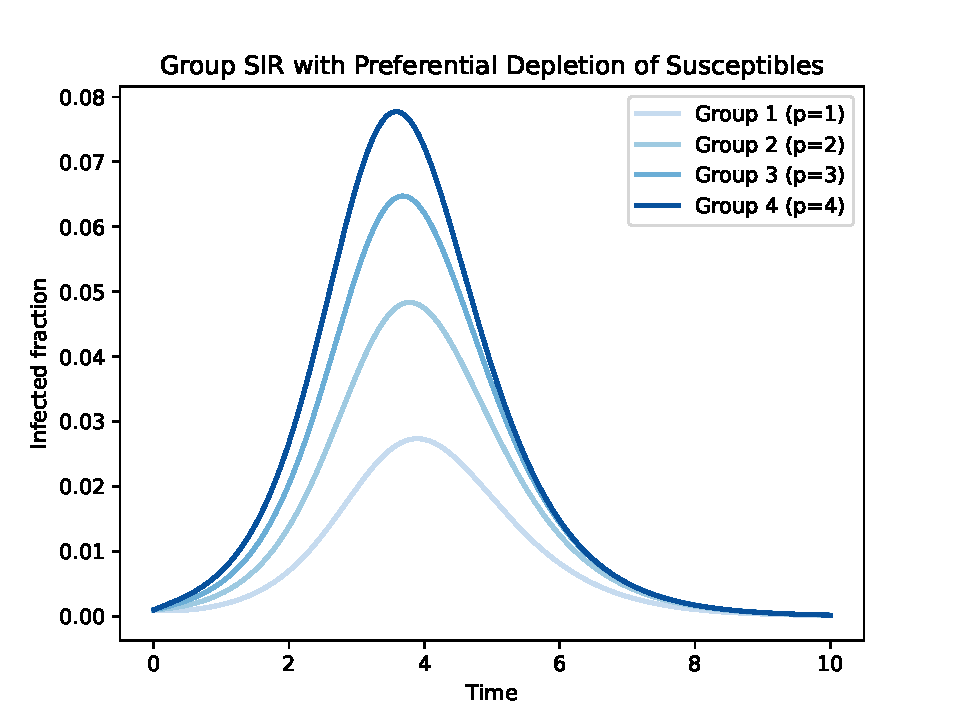
\includegraphics[width=0.5\textwidth]{1d.pdf}
		\caption{Preferential depletion of susceptibles across groups.}
		\label{fig:preferential_depletion}
	\end{figure}
	
	\item Define the average relative susceptibility among the susceptibles at any point in time $\bar{p}(t)$ as
%	$$\bar{p}(t) = \frac{\displaystyle \sum_{i=1}^4 p_i\,s_i(t)}{\displaystyle \sum_{i=1}^4 s_i(t)}\ .$$
	$$\bar{p}(t) = \displaystyle \sum_{i=1}^4 p_i\,s_i(t) \Bigg / \displaystyle \sum_{i=1}^4 s_i(t)\ .$$
	Note that this is simply a weighted average of the susceptibilities of the susceptibles, by adding up the susceptibilities in the numerator and dividing by the number of susceptibles in the denominator. Over the same time window as your previous plot, create two addition figures: First, show $s_i(t)$ for each $i=1, 2, 3, 4$ using the same color scheme as before. Second, show $\bar{p}(t)$ in black. 
	\begin{figure}[H]
		\centering
		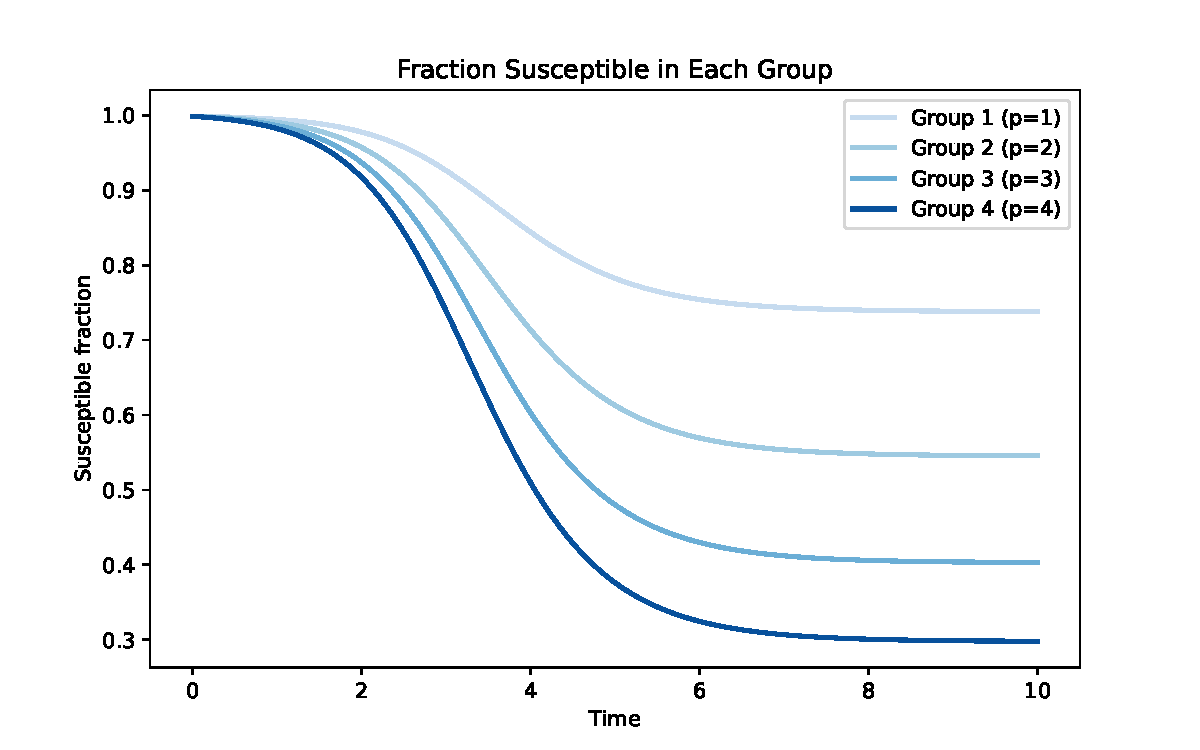
\includegraphics[width=0.5\textwidth]{1e1.pdf}
		\caption{Fraction of susceptibles.}
		\label{fig:sus_fraction}
	\end{figure}
	\begin{figure}[H]
		\centering
		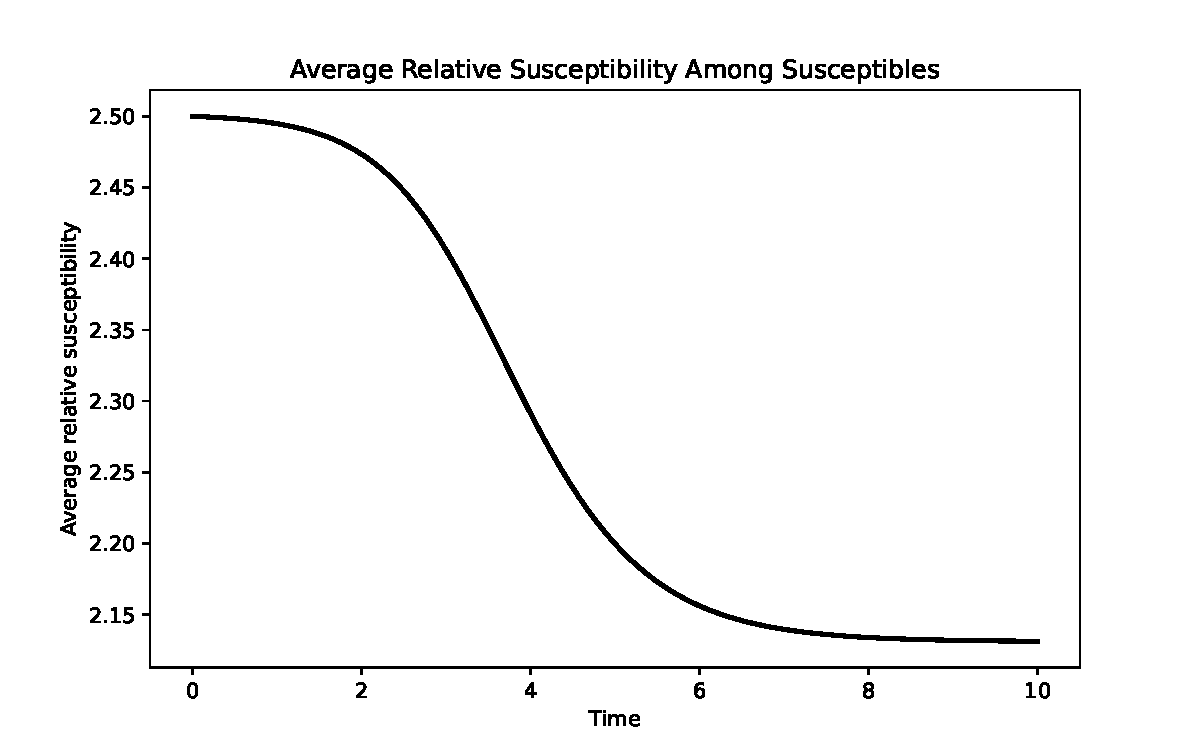
\includegraphics[width=0.5\textwidth]{1e2.pdf}
		\caption{Average relative susceptibility.}
		\label{fig:rel_sus}
	\end{figure}
	\item Comment on what you observe in the plots, and explain the reason for the patterns in words that a high school student could understand.
	\par
	\textbf{Answer:} In Figure \ref{fig:preferential_depletion}, we see that all groups have a wave-shaped infection curve where some peaks are higher than others.
	This is because some people can get sick easier than others (Group 4), which leads to more of these people getting infected.
	In Figure \ref{fig:sus_fraction}, we see that some groups lose most of its susceptible fraction more than others depending on how easily they can get sick.
	Group 4 gets sick the easiest, and therefore more of these people will get sick first. Comparing it to group 1, these people get sick the last and so they get infected a lot less.
	In figure \ref{fig:rel_sus} we see that the average at the start is 2.5 and then it decreases to 2.1. This is because at the start, everyone can get infected, but some groups are easier to infect than others. The disease spreads fastest in these highly susceptible groups, so they get sick first and recover, leaving behind people who are harder to infect. Over time, this makes the average susceptibility among the remaining susceptible people go down.
	\item[Grad/EC] Reflect on these plots in the context of the COVID-19 pandemic. What lessons are there to be drawn from the relationship between an epidemic wave and different groups with different susceptibilities?
	\par
	\textbf{Answer:} In the pandemic, not everyone is equally likely to get infected which means they all have different risks to the pandemic.
	Older adults or people with health conditions were more susceptible and therefore at higher risk and would be the first and hardest to be hit.
	Knowing this, it is important to place legislation, control measures, and vaccination strategies that protect those who are most at risk first.
\end{enumerate}
\clearpage

\item The goal of this problem is to explore branching processes, and how superspreading can, perhaps surprisingly, increase the likelihood that an outbreak never grows to a large size.

This problem introduces the {\bf negative binomial} (NB) distribution. The distribution can be parameterized a few different ways, but for our purposes, it will be convenient to specify a mean and a dispersion. In the context of transmission chains and branching processes, drawing the number of secondary infections from a negative binomial requires that the mean be $R_0$. However, the dispersion parameter allows us flexibility, and importantly, allows us to model superspreading. 

When $k \to \infty$, the negative binomial distribution converges to a Poisson distribution. When $k = 1$, the negative binomial is equivalent to a geometric distribution. A key difference between these is that the mode of a Poisson---its most common value---is around its mean, while the mode of a Geometric is zero. In the context of branching processes, this means that a high $k$ will lead to more similar numbers of secondary infections for each primary infection. In contrast, a low $k$ will lead to many instances where there are just a few (or zero) secondary infections, and rare instances with a large number of secondary infections. When $k$ is low, we often talk about ``superspreaders,'' people whose infections lead to an exceptionally larger number of secondary infections. 

Note: You can find Python code to draw from a negative binomial with the $R_0$ and $k$ parameterization provided on the next page. For those writing in other languages, be careful to use the correct parameterization (mean and dispersion).

\begin{enumerate}[label=\alph*.]
	\item Write code for a branching process that, starting from a single infection, draws $G$ generations, with each infection creating $NB(R_0,k)$ additional infections. Use your code to estimate $q$ the probability\footnote{See class notes.} that an epidemic dies in finite time, for $R_0=3$ and $k=0.1, 0.5, 1.0, 5.0,$ and $10.0$.\footnote{Hint: When we estimate a probability from a stochastic process like this, a convenient way to do this is Monte Carlo: simulate, say, $100,000$ branching processes and take note of how many cease before growing large.} Provide your answers in a table, out to 3 decimal places.
	\par
	\textbf{Answer: } \href{https://github.com/ctrlaltaf/csci57897-2/blob/main/code.ipynb}{Here is the link to my code}
	\begin{table}[H]
		\centering
		\caption{Estimated extinction probabilities $q$ for different dispersion parameters $k$ 
		in a branching process with $R_0 = 3$}
		\label{tab:extinction_probabilities}
		\begin{tabular}{c c c}
		\hline
		\textbf{Dispersion ($k$)} & \textbf{Extinction Probability ($q$)} & \textbf{Runtime (s)} \\ 
		\hline
		0.1  & 0.837 & 4.13 \\
		0.5  & 0.499 & 16.89 \\
		1.0  & 0.337 & 14.75 \\
		5.0  & 0.117 & 21.94 \\
		10.0 & 0.088 & 22.48 \\
		\hline
		\end{tabular}
	\end{table}
	\item How does $k$ affect $q$? Explain what this means in terms of the relationship between $p$ (i.e., $1-q$) and superspreading. 
	\par
	\textbf{Answer: }As k increases, the extinction probability q decreases. When k is small, the population shows strong superspreading. Most infected individuals cause few or no secondary infections, but a few cause many.
	When k is large , infections are more uniform since everyone infects about the same number of others so outbreaks are more likely to keep growing, and q becomes smaller
	\item [Grad/EC] How large do finite outbreaks get before they die out? For the parameters above, and for only the {\it finite} outbreaks, plot a histogram of $100,000$ finite outbreaks for your choice or choices of $k$, and $R_0=3$. What do you observe? 
	\par
	\textbf{Answer: } For smaller values of k, we see that there are total outbreak sizes that are shifted more on the left, and fewer outbreaks as the size increases.
	This left skew moves more to the right for larger values of k, which indicate that there are more finite outbreaks of larger size.
	\begin{figure}[H]
		\centering
		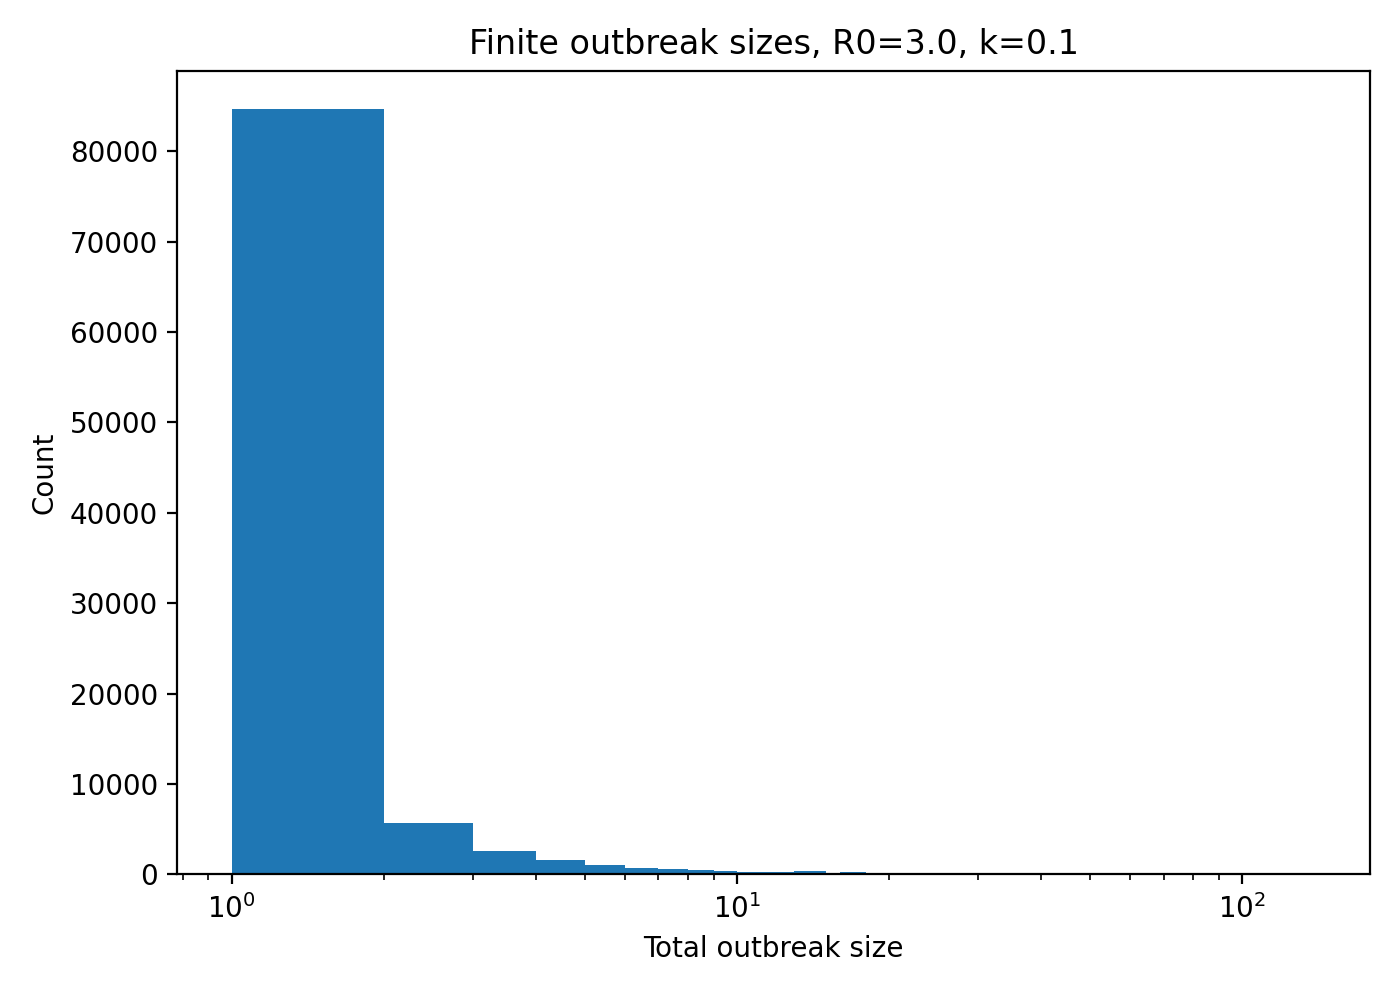
\includegraphics[width=0.5\textwidth]{finite_sizes_R03_k0.1.png}
		\caption{Finite outbreaks k = 0.1}
		\label{fig:k_0.1}
	\end{figure}
	\begin{figure}[H]
		\centering
		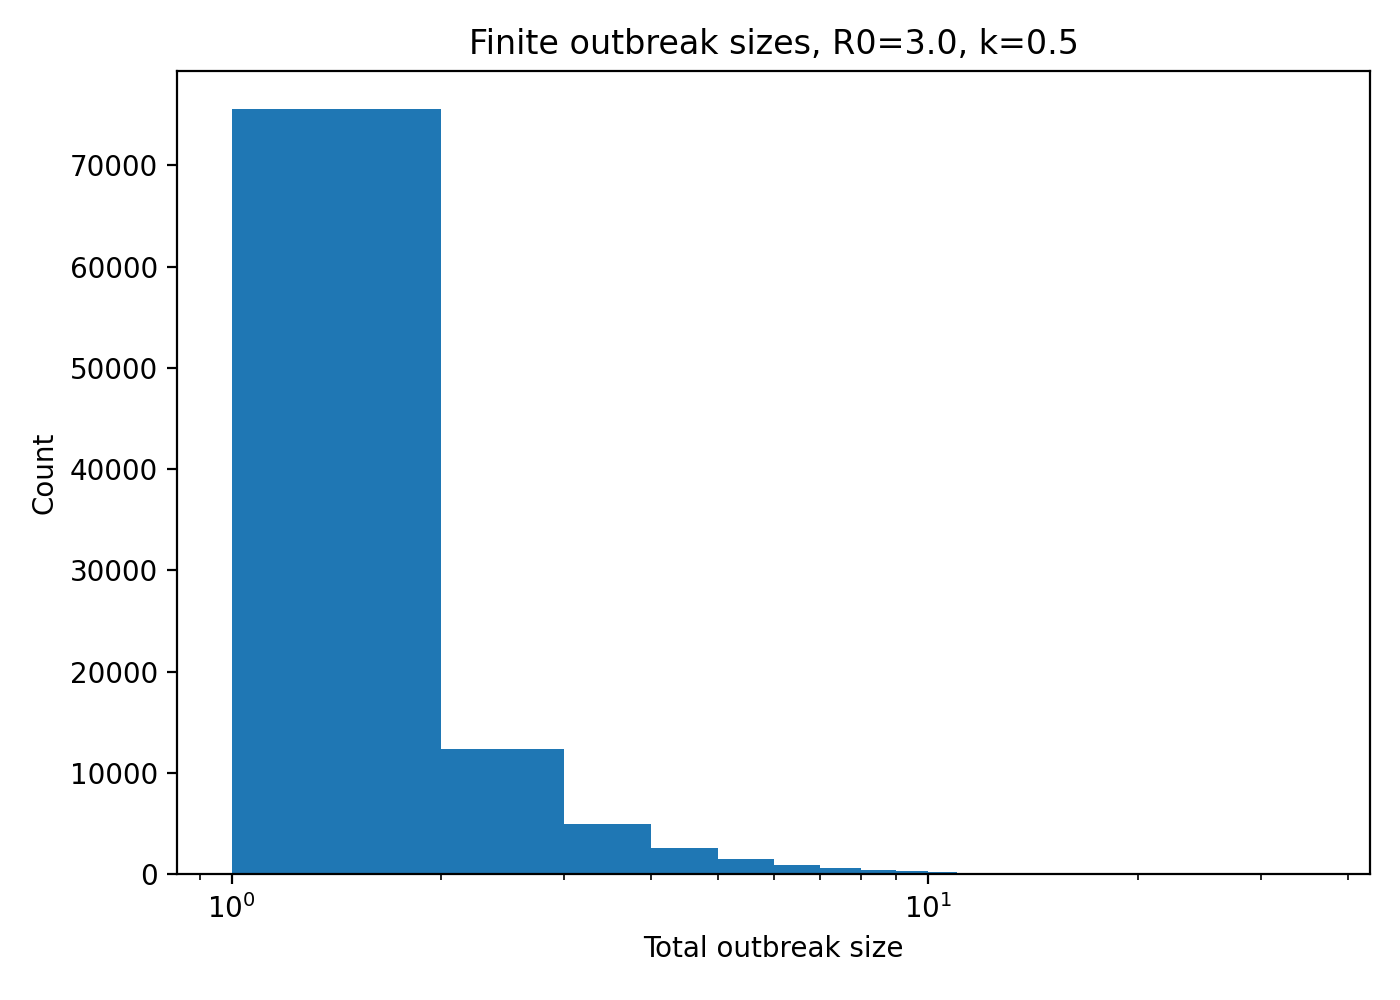
\includegraphics[width=0.5\textwidth]{finite_sizes_R03_k0.5.png}
		\caption{Finite outbreaks k = 0.5}
		\label{fig:k_0.5}
	\end{figure}
	\begin{figure}[H]
		\centering
		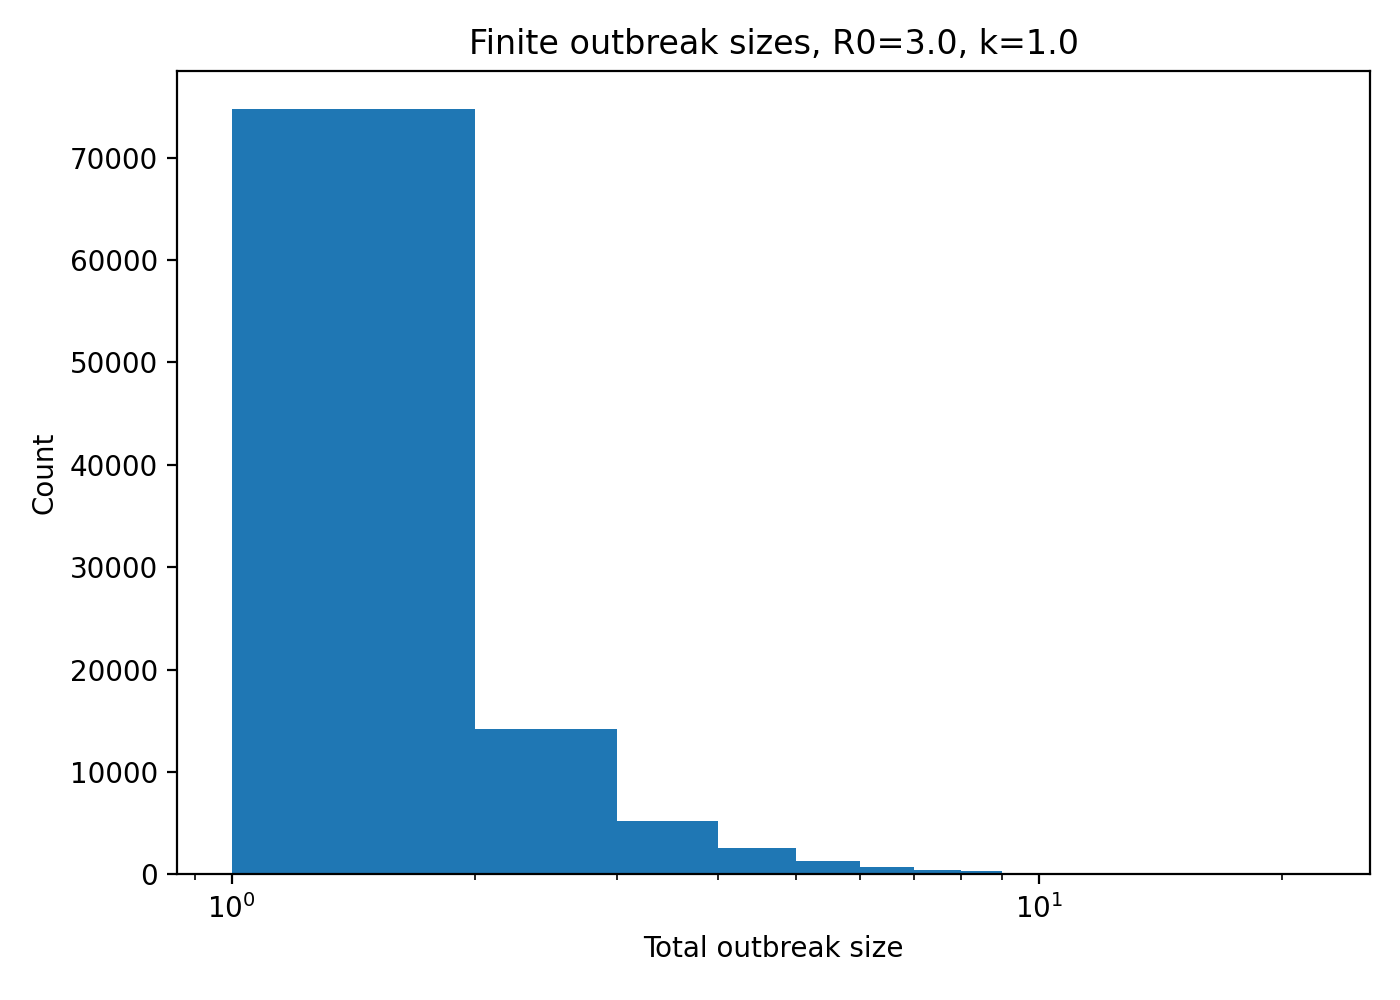
\includegraphics[width=0.5\textwidth]{finite_sizes_R03_k1.0.png}
		\caption{Finite outbreaks k = 1}
		\label{fig:k_1}
	\end{figure}
	\begin{figure}[H]
		\centering
		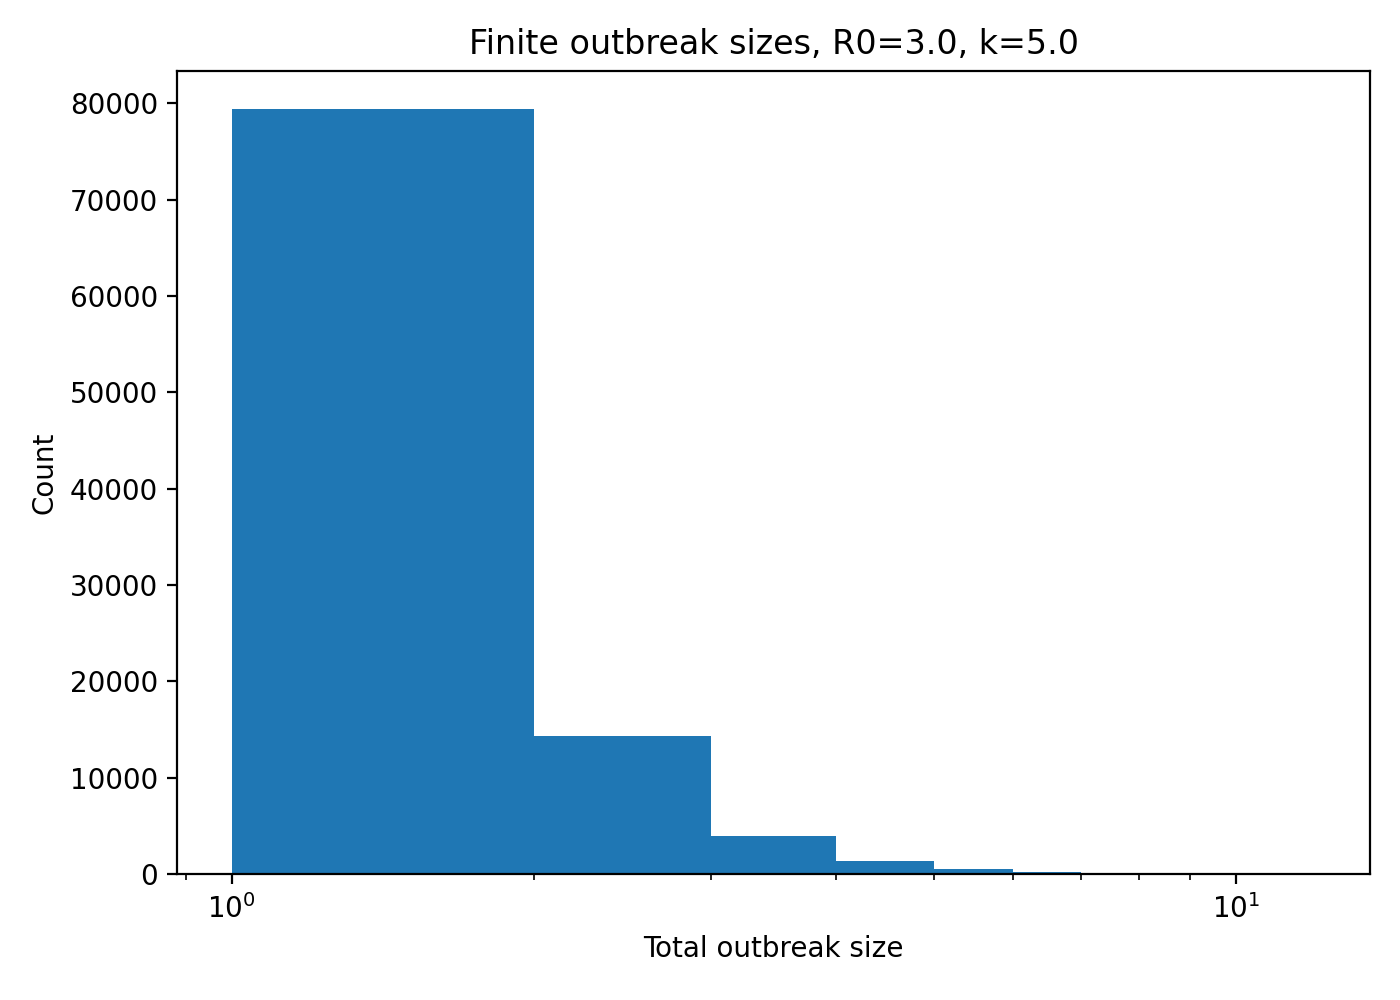
\includegraphics[width=0.5\textwidth]{finite_sizes_R03_k5.0.png}
		\caption{Finite outbreaks k = 5}
		\label{fig:k_5}
	\end{figure}
	\begin{figure}[H]
		\centering
		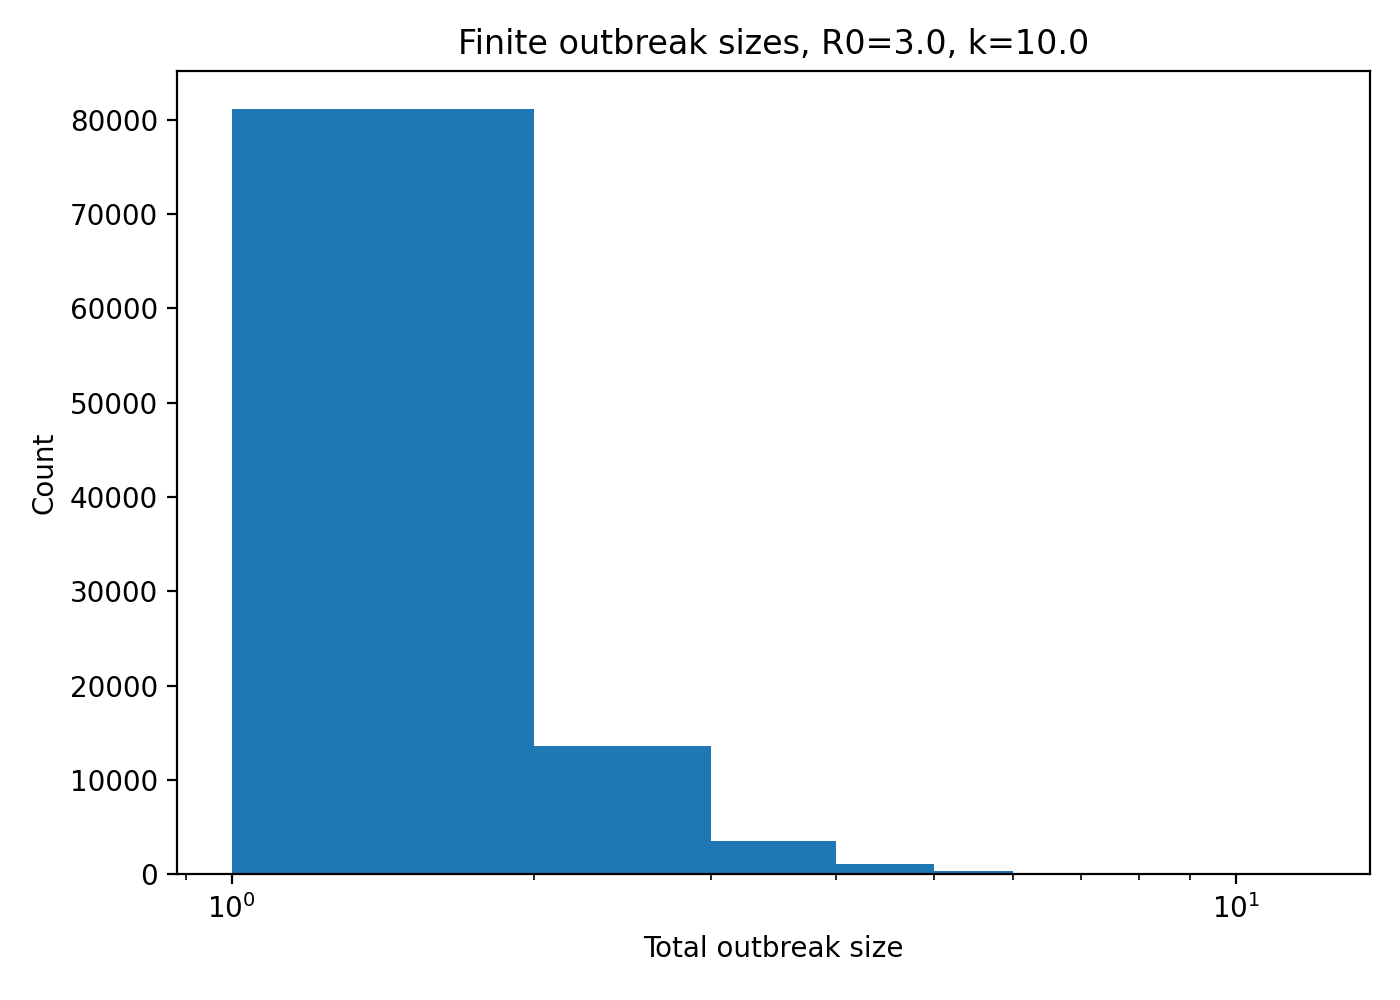
\includegraphics[width=0.5\textwidth]{finite_sizes_R03_k10.0.png}
		\caption{Finite outbreaks k = 10}
		\label{fig:k_10}
	\end{figure}
\end{enumerate}

\clearpage
Here is some Python code to draw from $NB(R_0, k)$:
\begin{verbatim}
from scipy.stats import nbinom

k = 10000 # Dispersion Parameter k
R0 = 3 # Mean R0

mean = R0
variance = mean + (mean**2)/k
p = mean/variance
n = mean**2 / (variance - mean) 

draw = nbinom.rvs(n=n,p=p)
draws = nbinom.rvs(n=n,p=p,size=10)
\end{verbatim}



\end{enumerate}

\end{document}